\documentclass[10pt,a4paper]{article}
\usepackage[utf8]{inputenc}
\usepackage{amsthm, amsmath, mathtools, amssymb}
\usepackage[left=2cm,right=2cm,top=2cm,bottom=2cm]{geometry}
\usepackage[colorlinks,linkcolor=blue,citecolor=blue,urlcolor=blue]{hyperref}
\usepackage[catalan]{babel}
\usepackage{titlesec}
\usepackage{enumitem}
\usepackage{physics}
\usepackage{fancyhdr}

\newcommand{\NN}{\ensuremath{\mathbb{N}}} % set of natural numbers
\newcommand{\ZZ}{\ensuremath{\mathbb{Z}}} % set of integers
\newcommand{\QQ}{\ensuremath{\mathbb{Q}}} % set of rationals
\newcommand{\RR}{\ensuremath{\mathbb{R}}} % set of real numbers
\newcommand{\CC}{\ensuremath{\mathbb{C}}} % set of complex numbers
\newcommand{\KK}{\ensuremath{\mathbb{K}}} % a general field

\newcommand{\vf}[1]{\boldsymbol{\mathrm{#1}}} % math style for vectors and matrices and vector-values functions (previously it was \*vb{#1} but this does not apply to greek letters)
\newcommand{\ii}{\mathrm{i}} % imaginary unit
\renewcommand{\O}{\mathrm{O}} % big O-notation


%%% PROBABILITY
\newcommand{\Prob}{\ensuremath{\mathbb{P}}} % probability
\newcommand{\Exp}{\mathbb{E}} % expected value
\newcommand{\Var}{\mathrm{Var}} % variance
\newcommand{\cov}{\mathrm{Cov}} % covariance
\newcommand{\iid}{i.i.d.} % independent and identically distributed
\newcommand{\indi}[1]{\vf{1}_{#1}}
\newcommand{\almoste}[1]{\overset{\text{a.e.}}{#1}} % almost everywhere


%%% STATISTICS
\DeclareMathOperator{\bias}{bias} % Bias
\DeclareMathOperator{\MSE}{MSE} % Mean Square Error
\DeclareMathOperator{\Mod}{Mod} % mode
\DeclareMathOperator{\Med}{Med} % median
\DeclareMathOperator*{\argmax}{arg\,max} % argument where the maximum is attained
\DeclareMathOperator*{\argmin}{arg\,min} % argument where the minimum is attained



\newtheorem{theorem}{Teorema}
\newtheorem{prop}{Proposició}
\newtheorem{exercici}{Exercici}
\theoremstyle{definition}
\newtheorem{definition}{Definició}
\theoremstyle{remark}
\newtheorem*{res}{Resolució}
\DeclareDocumentCommand\derivative{ s o m g d() }{ 
  % Total derivative
  % s: star for \flatfrac flat derivative
  % o: optional n for nth derivative
  % m: mandatory (x in df/dx)
  % g: optional (f in df/dx)
  % d: long-form d/dx(...)
    \IfBooleanTF{#1}
    {\let\fractype\flatfrac}
    {\let\fractype\frac}
    \IfNoValueTF{#4}
    {
        \IfNoValueTF{#5}
        {\fractype{\diffd \IfNoValueTF{#2}{}{^{#2}}}{\diffd #3\IfNoValueTF{#2}{}{^{#2}}}}
        {\fractype{\diffd \IfNoValueTF{#2}{}{^{#2}}}{\diffd #3\IfNoValueTF{#2}{}{^{#2}}} \argopen(#5\argclose)}
    }
    {\fractype{\diffd \IfNoValueTF{#2}{}{^{#2}} #3}{\diffd #4\IfNoValueTF{#2}{}{^{#2}}}\IfValueT{#5}{(#5)}}
} % differential operator
\DeclareDocumentCommand\partialderivative{ s o m g d() }{ 
  % Total derivative
  % s: star for \flatfrac flat derivative
  % o: optional n for nth derivative
  % m: mandatory (x in df/dx)
  % g: optional (f in df/dx)
  % d: long-form d/dx(...)
  \IfBooleanTF{#1}
    {\let\fractype\flatfrac}
    {\let\fractype\frac}
    \IfNoValueTF{#4}{
      \IfNoValueTF{#5}
      {\fractype{\partial \IfNoValueTF{#2}{}{^{#2}}}{\partial #3\IfNoValueTF{#2}{}{^{#2}}}}
      {\fractype{\partial \IfNoValueTF{#2}{}{^{#2}}}{\partial #3\IfNoValueTF{#2}{}{^{#2}}} \argopen(#5\argclose)}
    }
    {\fractype{\partial \IfNoValueTF{#2}{}{^{#2}} #3}{\partial #4\IfNoValueTF{#2}{}{^{#2}}}\IfValueT{#5}{(#5)}}
} % partial differential operator

\titleformat{\section}
  {\normalfont\fontsize{11}{15}\bfseries}{\thesection}{1em}{}

\renewcommand{\theenumi}{\textbf{\arabic{enumi}}}
\renewcommand{\theenumii}{\textbf{\alph{enumii}}}
\renewcommand{\theenumiii}{\textbf{\roman{enumiii}}}

\renewcommand{\exp}[1]{\mathrm{e}^{#1}} % exponential function
\DeclareMathOperator*{\im}{Im}

\title{\bfseries\Large Seminari 1\\Processos de Ramificació}

\author{Víctor Ballester Ribó\\NIU: 1570866}
\date{\parbox{\linewidth}{\centering
  Processos estocàstics\endgraf
  Grau en Matemàtiques\endgraf
  Universitat Autònoma de Barcelona\endgraf
  Març de 2023}}
  \pagestyle{fancy}
  \fancyhf{}
  \fancyhfoffset[L]{1cm}
  \fancyhfoffset[R]{1cm}
  \rhead{NIU: 1570866}
  \lhead{Víctor Ballester}
  \cfoot{\thepage}
  %\setlength{\headheight}{13.6pt}

\setlength{\parindent}{0pt}
\begin{document}
\selectlanguage{catalan}
\maketitle
\begin{exercici}
  Considerem dos punts $A:=(a,\alpha)$ i $B:=(b,\beta)$ tals que $b>a\geq 0$ i $\alpha,\beta>0$, tots ells naturals. Definim la reflexió de $A$ en l'eix horizontal $t$ com el punt $A':=(a,-\alpha)$. Justifiqueu el resultat següent.

  Principi de reflexió: el nombre de trajectòries de $A$ a $B$ que toquen o creuen l'eix $t$ és igual al nombre de trajectòries de $A'$ a $B$.
\end{exercici}
\begin{res}
  Cal veure que hi ha una bijecció entre el conjunt de trajectòries de $A$ a $B$ que toquen o creuen l'eix $t$ i el conjunt de trajectòries de $A'$ a $B$. Sigui $s=(s_a,s_{a+1},\ldots,s_b)$ una trajectòria de $A$ a $B$ que toca o creua l'eix. Llavors $\exists k\in\{a,\ldots,b-1\}$ tal que $s_k=0$. Ara si considerem la trajectòria $$s'=(-s_a,-s_{a+1},\ldots,-s_{k-1},s_k,s_{k+1},\ldots,s_b)$$ tenim que $s'$ és una trajectòria de $A'$ a $B$ ja que per construcció no em perdut la continuïtat i també per construcció cada $s_j$ difereix en una unitat dels seus veïns $s_{j-1}$ i $s_{j+1}$.

  Recíprocament, si $s=(s_a,s_{a+1},\ldots,s_b)$ és una trajectòria de $A'$ a $B$, aleshores pel teorema de Bolzano existeix $k\in\{a,\ldots,b-1\}$ tal que $s_k=0$. Ara si considerem la trajectòria $$s'=(-s_a,-s_{a+1},\ldots,-s_{k-1},s_k,s_{k+1},\ldots,s_b)$$ tenim que $s'$ és una trajectòria de $A$ a $B$ (pel mateix argument que abans) que toca o creua l'eix $t$ (almenys en $(k,s_k)$).

  \begin{figure}[ht]
    \centering
    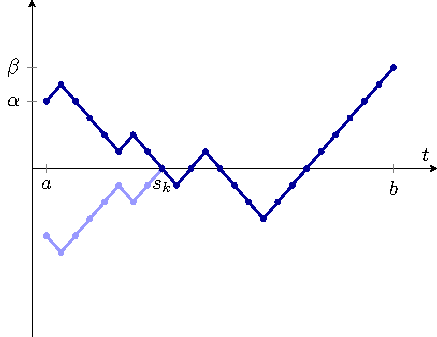
\includegraphics[width=0.5\textwidth]{Images/trajectoria.pdf}
    \caption{Exemple de trajectòries de $A$ a $B$ que toquen o creuen l'eix $t$ i de $A'$ a $B$.}
  \end{figure}
\end{res}
\begin{exercici}
  Demostreu el teorema de la votació: sigui $n$ i $x$ enters positius tals que existeixen dos enters positius $n_1$ i $n_2$ tals que $n_1 + n_2 = n$ i $n_1-n_2=x$. Definim $N_{n,x}=\binom{n}{n_1}$. Proveu que existeixen exactament $\frac{x}{n}N_{n,x}$ trajectòries $(0,s_1,\ldots,s_{n-1},x)$ tals que van de l'origen al punt $(n,x)$ i són tals que $s_1,\ldots,s_{n-1}>0$.

  Com a aplicació, suposem que en una votació amb dos partits, A i B, el partit A ha tret $n_1$ vots i el partit B $n_2$ vots amb $n_1 > n_2$ . Quina és la probabilitat que en tot moment de l'escrutini el partit A vagi per endavant? Feu el cas concret $n_1=1200$ i $n_2=800$.
\end{exercici}
\begin{res}
  Fixem-nos que el nombre de trajectòries per anar de l'origen al punt $(n,x)$ és $N_{n,x}$. En efecte, si usem $n_1$ passos cap endavant (i.e positius o cap amunt en la figura anterior) i $n_2$ passos cap endarrera (i.e. negatius o cap avall) aleshores tenim que el nombre de trajectòries vindrà determinat un cop co\lgem oquem les posicions dels passos positius, que podem fer-ho de $\binom{n}{n_1}=N_{n,x}$ maneres diferents.

  Fixem-nos que el que ens demanen és equivalent a comptar el nombre de trajectòries $(1,s_2,\ldots,s_{n-1},x)$ que van des del punt $(1,1)$ al punt $(n,x)$ i són tals que $s_2,\ldots,s_{n-1}>0$ (ja que si des de l'origen no volem tocar l'eix només podem anar cap amunt), que a la vegada és el nombre total de trajectòries que van des del punt $(1,1)$ al punt $(n,x)$ menys el nombre de trajectòries que van des del punt $(1,1)$ al punt $(n,x)$ i tallen o toquen l'eix $t$. El primer terme d'aquests dos és $N_{n-1,x-1}=\binom{n-1}{\tilde{n}_1}=\binom{n-1}{n_1-1}$ ja que $\tilde{n}_1$ i $\tilde{n}_2$ satifan:
  $$
    \begin{cases}
      \tilde{n}_1+\tilde{n}_2=n-1 \\
      \tilde{n}_1-\tilde{n}_2=x-1
    \end{cases}\iff
    \begin{cases}
      2\tilde{n}_1=n+x-2 \\
      2\tilde{n}_2=n-x
    \end{cases}
    \iff
    \begin{cases}
      2\tilde{n}_1=2n_1-2 \\
      2\tilde{n}_2=2n_2
    \end{cases}
    \iff
    \begin{cases}
      \tilde{n}_1=n_1-1 \\
      \tilde{n}_2=n_2
    \end{cases}
  $$
  Per calcular el segon terme usem l'exercici 1 i calculem el nombre de trajectòries que van des de $(1,-1)$ a $(n,x)$. Aquest nombre és $N_{n-1,x+1}=\binom{n-1}{\bar{n}_1}=\binom{n-1}{n_1}$ ja que $\bar{n}_1$ i $\bar{n}_2$ satifan:
  $$
    \begin{cases}
      \bar{n}_1+\bar{n}_2=n-1 \\
      \bar{n}_1-\bar{n}_2=x+1
    \end{cases}\iff
    \begin{cases}
      2\bar{n}_1=n+x \\
      2\bar{n}_2=n-x+2
    \end{cases}
    \iff
    \begin{cases}
      2\bar{n}_1=2n_1 \\
      2\bar{n}_2=2n_2-2
    \end{cases}
    \iff
    \begin{cases}
      \bar{n}_1=n_1 \\
      \bar{n}_2=n_2-1
    \end{cases}
  $$
  Per tant, el valor que ens demana l'exercici és:
  $$\binom{n-1}{n_1-1}-\binom{n-1}{n_1}=\frac{n!}{(n-n_1)!n_1!}\left(\frac{n_1}{n}-\frac{n-n_1}{n}\right)=\binom{n}{n_1}\frac{2n_1-n}{n}=\frac{x}{n}\binom{n}{n_1}=\frac{x}{n}N_{n,x}$$

  La segona part és una simple aplicació del que hem fet. Si pensem que els vots al partit A són passos positius en la nostra trajectòria i els vots al partit B són passos negatius, aleshores el que ens demanen és el nombre de trajectòries que van des de $(0,0)$ a $(n_1+n_2,n_1-n_2)$ i que sempre estan estrictament per sobre l'eix $t$. Aquest nombre és:
  $$\frac{x}{n}N_{n,x}=\frac{400}{2000}N_{n,x}=\frac{1}{5}N_{n,x}$$
  I la probabilitat que sempre estiguin per sobre l'eix $t$ és: $$\frac{\frac{1}{5}N_{n,x}}{N_{n,x}}=\frac{1}{5}$$
  ja que recordem que $N_{n,x}$ és el nombre total de trajectòries que van des de $(0,0)$ a $(n_1+n_2,n_1-n_2)$.
\end{res}
\begin{exercici}
  Donat un passeig aleatori simple, sortint de 0, calculeu la probabilitat de visitar alguna vegada l'estat $b$, on $b$ és un enter estrictament positiu.
\end{exercici}
\begin{res}
  Sigui $(X_n)_{n\geq 1}$ variables aleatòries tals que $\Prob(X_n=1)=p$ i $\Prob(X_n=-1)=q$ i $X_0=0$ independent de totes les altres. Sigui $S_n=\sum_{i=0}^n X_i$ un passeig aleatori simple. Volem calcular $\Prob(D)$ on $\displaystyle D=\{\exists n\in\NN \cup\{0\}:S_n=b\}$. Per això definim $C_z$ com $$C_z:=\{\exists n\in\NN\cup\{0\}:S_n=b\text{ i }S_m>-z,m=0,\ldots,n-1\}$$
  Fixem-nos que $\Prob(C_z)$ és exactament la probabilitat d'arruïnar el nostre contrincant en el joc de la ruïna del jugador fent la translació $b=a-z$ (usant la notació de classe). Per tant, usant les fórmules que vam demostrar:
  $$
    \Prob(C_z)=\begin{cases}
      \frac{-{\left(\frac{p}{q}\right)}^a+{\left(\frac{p}{q}\right)}^{a-z}}{1-{\left(\frac{p}{q}\right)}^a} & \text{si $p\ne 1/2$} \\
      \frac{z}{a}                                                                                           & \text{si $p= 1/2$}
    \end{cases}=\begin{cases}
      \frac{-{\left(\frac{p}{q}\right)}^{b+z}+{\left(\frac{p}{q}\right)}^{b}}{1-{\left(\frac{p}{q}\right)}^{b+z}} & \text{si $p\ne 1/2$} \\
      \frac{z}{b+z}                                                                                               & \text{si $p= 1/2$}
    \end{cases}
  $$
  Notem que $C_z\subseteq C_{z+1}$, ja que si $S_m>-z$ aleshores també tindrem $S_m>-(z+1)$ $\forall m=0,\ldots,n-1$. D'altra banda notem que $D=\bigcup_{z=0}^\infty C_z$. En efecte, tenim que si $\exists n\in\NN\cup\{0\}$ de manera que $S_n=b$ aleshores prenent $\ell:=\min_{m=0,\ldots,n-1}S_m$ tenim que $n$ també satisfà la condició de l'esdeveniment $C_{\ell+1}$. I per tant, està a la unió $\bigcup_{z=0}^\infty C_z$. L'altra inclusió és clara ja que cada $C_z\subseteq D$. Per tant, pel lema de les unions creixents tenim que $\displaystyle \Prob(D)=\lim_{z\to\infty}\Prob(C_z)$. Aquest límit és fàcilment calculable i dona:
  $$
    \Prob(D)=\lim_{z\to\infty}\begin{cases}
      \frac{-{\left(\frac{p}{q}\right)}^{b+z}+{\left(\frac{p}{q}\right)}^{b}}{1-{\left(\frac{p}{q}\right)}^{b+z}} & \text{si $p\ne 1/2$} \\
      \frac{z}{b+z}                                                                                               & \text{si $p= 1/2$}
    \end{cases}=\begin{cases}
      {\left(\frac{p}{q}\right)}^{b} & \text{si $p< 1/2$}    \\
      1                              & \text{si $p\geq 1/2$} \\
    \end{cases}
  $$
\end{res}
\begin{exercici}
  Suposem que dos jugadors A i B, amb fortuna conjunta $a$ (amb $a \in \NN$), juguen partides en què A pot guanyar una unitat (que perd B) amb probabilitat $p$, B pot guanyar una unitat amb probabilitat $q$ i poden empatar (llavors no guanya res cap dels dos) amb probabilitat $r$. Suposem que aquestes probabilitats són estrictament positives i que $p + q + r = 1$. Suposem que les successives partides són independents. Definim $u(i)$ com la probabilitat que A guanyi el joc (és a dir, B s'arruïna), suposant que la fortuna inicial del jugador A fossin i unitats. Deduïu una equació en diferències per a $u(i)$.
  Resoleu aquesta equació, amb les condicions frontera adequades i calculeu la probabilitat que A guanyi el joc si la seva fortuna inicial eren z unitats.
\end{exercici}
\begin{res}
  Sigui $(X_n)_{n\geq 1}$ les variables aleatòries que simulen cada partida. Per tant, $X_n$ pot prendre els valors $1$, $-1$, $0$ amb probabilitats $p$, $q$, $r$ respectivament. Tenim que de forma similar a la ruïna del jugador:
  \begin{multline*}
    \Prob(\text{$A$ guanya amb fortuna inicial $i$})=\Prob(\text{$A$ guanya amb fortuna inicial $i$}\mid X_1=1)p+\\+\Prob(\text{$A$ guanya amb fortuna inicial $i$}\mid X_1=-1)q+\Prob(\text{$A$ guanya amb fortuna inicial $i$}\mid X_1=0)r=\\=
    \Prob(\text{$A$ guanya amb fortuna inicial $i+1$})p+\Prob(\text{$A$ guanya amb fortuna inicial $i-1$})q+\\+\Prob(\text{$A$ guanya amb fortuna inicial $i$})r
  \end{multline*}
  Escrit en forma de recurrència tenim que:
  $$u(i)=u(i+1)p+u(i-1)q+u(i)r\implies u(i+1)+u(i)\frac{r-1}{p}+u(i-1)\frac{q}{p}=0$$
  El polinomi característic d'aquesta equació és $x^2+\frac{r-1}{p}x+\frac{q}{p}=0$, les arrels del qual són 1 i $\frac{q}{p}$. Fixem-nos que si $p=q$, aleshores les arrels són linealment dependents, però llavors és fàcil veure que hi ha una altra solució linealment independent de $u(i)=1$, que és $u(i)=i$. Per tant, la solució general és:
  $$
    \begin{cases}
      u(i)=c_1+c_2{\left(\frac{q}{p}\right)}^i & \text{si $p\ne q$} \\
      u(i)=c_1+c_2i                            & \text{si $p=q$}
    \end{cases}
  $$
  Les condicions de frontera són $u(0)=0$ i $u(a)=1$, ja que si $i=0$ aleshores $A$ no té fortuna i per tant no pot guanyar i si $i=a$ aleshores $A$ té tota la fortuna i per tant ja ha guanyat. Per tant, tenim que per $p\ne q$:
  $$
    \begin{cases}
      c_1+c_2=0 \\
      c_1+c_2{\left(\frac{q}{p}\right)}^a=1
    \end{cases}\implies
    c_2=-\frac{1}{1-{\left(\frac{q}{p}\right)}^a}\quad\text{i}\quad c_1=\frac{1}{1-{\left(\frac{q}{p}\right)}^a}
  $$
  I per $p=q$:
  $$
    \begin{cases}
      c_1=0 \\
      c_1+c_2a=1
    \end{cases}\implies
    c_1=0\quad\text{i}\quad c_2=\frac{1}{a}
  $$
  Finalment la solució és:
  $$u(z)=
    \begin{cases}
      \frac{1-{\left(\frac{q}{p}\right)}^z}{1-{\left(\frac{q}{p}\right)}^a} & \text{si $p\ne q$} \\
      \frac{z}{a}                                                           & \text{si $p=q$}
    \end{cases}
  $$
  que no depèn de $r$.
\end{res}
\end{document}
